\documentclass[11pt,reqno]{amsart}

\usepackage[T1]{fontenc}
\usepackage{lmodern}
\usepackage{amsmath,amssymb,amsthm,mathtools}
\usepackage{booktabs}
\usepackage{graphicx}
\usepackage{enumitem}
\usepackage[margin=1.15in]{geometry}
\usepackage{microtype}
\emergencystretch=1.5em
\usepackage[dvipsnames]{xcolor}
\usepackage[colorlinks=true,linkcolor=MidnightBlue,citecolor=MidnightBlue,urlcolor=MidnightBlue]{hyperref}

\newtheorem{theorem}{Theorem}[section]
\newtheorem{proposition}[theorem]{Proposition}
\newtheorem{lemma}[theorem]{Lemma}
\newtheorem{corollary}[theorem]{Corollary}
\theoremstyle{definition}
\newtheorem{definition}[theorem]{Definition}
\theoremstyle{remark}
\newtheorem{remark}[theorem]{Remark}

\numberwithin{equation}{section}

\newcommand{\R}{\mathbb{R}}
\newcommand{\C}{\mathbb{C}}
\newcommand{\N}{\mathbb{N}}
\newcommand{\Z}{\mathbb{Z}}
\newcommand{\dd}{\mathrm{d}}
\newcommand{\ii}{\mathrm{i}}
\newcommand{\ee}{\mathrm{e}}
\newcommand{\Rea}{\mathrm{Re}}
\newcommand{\Ima}{\mathrm{Im}}

\title[Poisson--Hadamard Inequalities and Quasiconcave Minorants]{Explicit Poisson--Hadamard Zero-Free Region Inequalities, Quasiconcave Minorant Crossing, Rigorous Trudgian Stieltjes Bounds, and Comparison with Smooth Weil Weights}

\author{Thijs Missiaen}
\address{Independent Researcher, Belgium (ORCID: \href{https://orcid.org/0009-0007-3678-0810}{0009-0007-3678-0810})}
\email{thijs.missiaen@gmail.com}
\date{November 2026}
\subjclass[2020]{Primary 11M06, 11M26; Secondary 30D15, 42A05}
\keywords{Riemann zeta function, explicit zero-free regions, Stechkin--Hadamard Poisson kernel, Fej\'er--Luk\'acs polynomials, Trudgian argument bound, Heath-Brown smooth weights}

\begin{document}

\begin{abstract}
We examine explicit de la Vall\'ee Poussin and Stechkin zero-free region inequalities for $\zeta(s)$ through the mirror-paired Hadamard Poisson kernel $K(d, \delta, u) = \frac{1}{2}[\frac{d-\delta}{(d-\delta)^2+u^2} + \frac{d+\delta}{(d+\delta)^2+u^2}]$ ($d > \frac{1}{2}$, $\delta = \lvert\beta - \frac{1}{2}\rvert \in [0, \frac{1}{2})$), connected to the canonical transverse Wronskian $W(d,t) = 16\int_0^{\infty} y\sinh(2dy)I(y,t)\,\dd y$. While $\int_{\R} K(d, \delta, u)\,\dd u = \pi$ is conserved, we prove that $K(d, \frac{1}{2}, u)$ is not a global minorant on $\R$: because $\delta^2 \mapsto K(d, \delta, u)$ is strictly quasiconcave on $[0, \frac{1}{4}]$, the sharp pointwise minorant is $K_{\flat}(d,u) = \min(K(d,0,u), K(d,\frac{1}{2},u))$ with crossing at $u_{\times}(d) < d/\sqrt{3}$, validating plateau minorants $\widetilde{K}_H(d,u)$ precisely for $H \ge u_{\times}(d)$. Incorporating Trudgian's unconditional bound $\lvert S(T)\rvert \le 0.112\ln T + 0.278\ln\ln T + 2.510$, logarithmic tail and concavity corrections, and focal-pair de-duplication at $u = 0$, we benchmark plateau subtraction against Mossinghoff--Trudgian--Yang ($R = 5.558691$) and explain why sharp Poisson truncation trails smooth Heath-Brown Weil weights.
\end{abstract}

\maketitle

\section{Introduction and Main Results}\label{sec:intro}

Under the canonical normalization established in Papers~V and~VI~\cite{missiaen2026p5,missiaen2026p6}, Riemann's $\Xi(z) := \xi(\frac{1}{2} + \ii z) = 8\int_0^{\infty} \Phi(u)\cos(2zu)\,\dd u$ ($z = t - \ii d$, $s = \frac{1}{2} + d + \ii t$)~\cite{riemann1859,jacobi1829,polya1926} has transverse Wronskian~\cite{speiser1934,lagarias1999,hinkkanen1997,csordas1986,wigner1932,hudson1974}
\begin{equation}\label{eq:W_canonical_p7}
W(d,t) := \frac{1}{2}\frac{\partial}{\partial d}\bigl\lvert\Xi(t - \ii d)\bigr\rvert^2 = \bigl\lvert\Xi(t - \ii d)\bigr\rvert^2\,\Rea\frac{\xi'(\frac{1}{2} + d + \ii t)}{\xi(\frac{1}{2} + d + \ii t)} = 16\int_0^{\infty} y\sinh(2dy)\,I(y,t)\,\dd y.
\end{equation}
For $d > \frac{1}{2}$ ($\sigma = \frac{1}{2} + d > 1$), $\Xi(t - \ii d) \ne 0$, and dividing $W(d, \tau)$ by $\lvert\Xi(\tau - \ii d)\rvert^2$ links Hadamard's zero-sum partial fraction $\Rea(\xi'/\xi)(s) = \sum_{\rho} \Rea(s - \rho)^{-1}$ directly to the Dirichlet series $-\Rea(\zeta'/\zeta)(s) = \sum_{n=2}^{\infty} \Lambda(n)n^{-1/2-d}\cos(\tau\ln n)$ via $\xi(s) = \frac{1}{2}s(s-1)\pi^{-s/2}\Gamma(s/2)\zeta(s)$.

Classical explicit zero-free regions---initiated by de la Vall\'ee Poussin~\cite{dlvp1899} and sharpened via functional-equation zero pairing by Stechkin~\cite{stechkin1970}, Kondratiev~\cite{kondratiev1977}, Heath-Brown~\cite{heathbrown1992}, and Mossinghoff, Trudgian, and Yang~\cite{mty2024}---combine non-negative trigonometric polynomials $P(\theta) = \frac{1}{2} + \sum_{k=1}^K w_k\cos(k\theta) \ge 0$ with lower bounds on the background nontrivial zero sum. Meanwhile, Platt and Trudgian~\cite{platttrudgian2021} verified unconditionally that every nontrivial zero with $\lvert\gamma\rvert \le 3 \cdot 10^{12}$ lies on $\sigma = \frac{1}{2}$, while Mossinghoff, Trudgian, and Yang~\cite{mty2024} established the classical region $\sigma \ge 1 - (5.558691\ln\lvert t\rvert)^{-1}$ ($\lvert t\rvert \ge 2$) and the asymptotically wider Korobov--Vinogradov~\cite{korobov1958,vinogradov1958} region $\sigma \ge 1 - [55.241(\ln\lvert t\rvert)^{2/3}(\ln\ln\lvert t\rvert)^{1/3}]^{-1}$ ($\lvert t\rvert \ge 3$).

This methodological note clarifies the exact algebra and analytical pitfalls of plateau-truncated Poisson--Hadamard background subtraction:

\begin{theorem}[Quasiconcave Minorant Crossing and Rigorous Plateau Stieltjes Bound]\label{thm:main_p7}
Let $d > \frac{1}{2}$, $\delta \in [0, \frac{1}{2}]$, and $K(d, \delta, u) := \frac{1}{2}[\frac{d-\delta}{(d-\delta)^2+u^2} + \frac{d+\delta}{(d+\delta)^2+u^2}]$.
\begin{enumerate}[label=\textup{(\roman*)},leftmargin=2.2em]
\item \textbf{Toeplitz Weight Bound and Stechkin Kernel Conservation.} Every degree-$K$ non-negative cosine polynomial $P(\theta) = \frac{1}{2} + \sum_{k=1}^K w_k\cos(k\theta) \ge 0$ satisfies $w_1 \le \cos(\frac{\pi}{K+2})$~\cite{fejer1916,szego1975}, with extremal sum $\sum_{k=1}^K w_k^{(K)} = \frac{1}{K+2}\cot^2(\frac{\pi}{2(K+2)}) - \frac{1}{2}$. For all $0 \le \delta < d$, $\int_{-\infty}^{\infty} K(d, \delta, u)\,\dd u = \pi$.
\item \textbf{Quasiconcave Endpoint Crossing.} Because $\int_{\R}[K(d,\delta,u) - K(d,\frac{1}{2},u)]\,\dd u = 0$, $K(d, \frac{1}{2}, u)$ is \emph{not} a minorant near $u = 0$. Instead, $\delta^2 \mapsto K(d, \delta, u)$ is strictly quasiconcave on $[0, \frac{1}{4}]$, so $\min_{\delta \in [0,1/2]} K(d, \delta, u) = \min(K(d,0,u), K(d,\frac{1}{2},u))$, crossing uniquely on $(0,\infty)$ at $u_{\times}(d) < d/\sqrt{3}$ in~\eqref{eq:u_cross_exact}. Consequently, $\widetilde{K}_H(d,u) := K(d, \frac{1}{2}, \max(\lvert u\rvert, H))$ is a valid global minorant on $\R$ whenever $H \ge u_{\times}(d)$.
\item \textbf{Rigorous Trudgian Stieltjes Lower Bound and Focal De-Duplication.} Using Trudgian's bound~\cite{trudgian2014} $\lvert S(T)\rvert \le B_S^{(0)}(T) := 0.112\ln T + 0.278\ln\ln T + 2.510$ ($T \ge \ee$), every ordinate $\tau \ge 30$ and $H \in [u_{\times}(d), \tau/2]$ satisfies the unconditional bound~\eqref{eq:rigorous_bg_bound}, where extracting a putative off-line pair $\{\rho_0, 1-\bar{\rho}_0\}$ at $\gamma = t$ requires subtracting $2K(d, \frac{1}{2}, H)$ at $k = 1$ to prevent $u = 0$ double counting. Because piecewise-smooth plateau corners incur Stieltjes boundary jumps $\approx 2B_S^{(0)}(\tau)K(d,\frac{1}{2},H)$, plateau Poisson subtraction yields $R_{\mathrm{eff}} > 5.558691$, trailing smooth compactly supported Fourier/Weil weights~\cite{heathbrown1992,mty2024}.
\end{enumerate}
\end{theorem}

\subsection{Proof overview}\label{subsec:proof_overview}

The proofs rely on three analytical steps:
\begin{enumerate}[label=\textup{(\arabic*)},leftmargin=2.2em]
\item \textit{Fej\'er--Riesz factorization and reflection bijection (Sections~\ref{sec:fejer}--\ref{sec:stechkin}).} Writing $P(\theta) = \frac{1}{2}\lvert\sum_{j=0}^K a_j\ee^{\ii j\theta}\rvert^2$ reduces $\max w_1$ to the tridiagonal Toeplitz eigenvalue $2\cos(\frac{\pi}{K+2})$, while the involution $\rho \mapsto 1 - \bar{\rho}$ pairs the multiset of nontrivial zeros into $K(d, d_\rho, \tau - \gamma)$ without miscounting on-line versus off-line multiplicities.
\item {\sloppy\textit{Biquadratic difference factorization and $\delta^2$-monotonicity (Section~\ref{sec:crossing}).} Factoring $K(d,\delta,u) - K(d,\frac{1}{2},u)$ isolates $3u^4 + (2d^2 + \frac{1}{4} + \delta^2)u^2 - (d^2 - \frac{1}{4})(d^2 - \delta^2)$, while $\partial_{\delta^2}K(d,\delta,u)$ changes sign at most once from $+$ to $-$, forcing the minimum onto $\{\delta = 0, \delta = \frac{1}{2}\}$.\par}
\item \textit{Stieltjes integration by parts with logarithmic tail and concavity control (Section~\ref{sec:trudgian}).} Bounding $B_S^{(0)}(\tau + u) - B_S^{(0)}(\tau + H) \le c_{\mathrm{tail}}(\tau+H)\ln(\frac{\tau+u}{\tau+H})$ closes the $[\tau+H, \infty)$ tail in elementary arctangents, while symmetric pairing on $[\tau - \frac{\tau}{2}, \tau + \frac{\tau}{2}]$ bounds concavity of $\ln(\gamma/2\pi)$ explicitly.
\end{enumerate}

\subsection{Notation and canonical normalizations}\label{subsec:notation}

Throughout, $s = \sigma + \ii\tau = \frac{1}{2} + d + \ii\tau$ with $d > \frac{1}{2}$ ($\sigma > 1$), $\mathcal{A}_\Gamma(d,\tau) := \frac{1}{2}\Rea\,\psi(\frac{1}{4} + \frac{d}{2} + \ii\frac{\tau}{2}) - \frac{1}{2}\ln\pi$, and nontrivial zeros $\rho = \beta + \ii\gamma$ have displacement $d_\rho := \lvert\beta - \frac{1}{2}\rvert \in [0, \frac{1}{2})$. Backlund's counting decomposition is $N(T) = \frac{1}{\pi}\vartheta(T) + 1 + S(T)$ for $T > 0$ ($N(14) = 0$ since $\gamma_1 \approx 14.134725$).

\section{Fej\'er--Luk\'acs Trigonometric Polynomials and Toeplitz Bounds}\label{sec:fejer}

\begin{proposition}[Fej\'er--Luk\'acs Eigenvalue Bound and Weight Sum~\cite{fejer1916,szego1975,kondratiev1977}]\label{prop:fejer_toeplitz}
Let $P(\theta) = \frac{1}{2} + \sum_{k=1}^K w_k\cos(k\theta) \ge 0$ for all $\theta \in \R$ ($w_k \in \R$, $K \ge 1$). Then there exist $a_0, \dots, a_K \in \R$ with $\sum_{j=0}^K a_j^2 = 1$ and $w_k = \sum_{j=0}^{K-k} a_j a_{j+k}$. Consequently,
\begin{equation}\label{eq:fejer_max_w1}
w_1 \le \frac{1}{2}\Lambda_{\max}(K) = \cos\!\left(\frac{\pi}{K+2}\right),
\end{equation}
attained uniquely (for $a_j \ge 0$) by $a_j^{(K)} := \sqrt{\frac{2}{K+2}}\sin\frac{(j+1)\pi}{K+2}$, for which
\begin{equation}\label{eq:cot_weight_sum}
\sum_{k=1}^K w_k^{(K)} = \frac{1}{K+2}\cot^2\!\left(\frac{\pi}{2(K+2)}\right) - \frac{1}{2}.
\end{equation}
\end{proposition}

\begin{proof}
By the Fej\'er--Riesz theorem~\cite[Thm.~1.2.1]{szego1975}, $2P(\theta) = \lvert\sum_{j=0}^K a_j\ee^{\ii j\theta}\rvert^2 = \sum_{j=0}^K a_j^2 + 2\sum_{k=1}^K (\sum_{j=0}^{K-k} a_j a_{j+k})\cos(k\theta)$, giving $\sum a_j^2 = 1$ and $2w_1 = a^{\mathsf{T}}J_K a$, where $J_K$ is the $(K+1) \times (K+1)$ tridiagonal shift matrix with eigenvalues $2\cos\frac{m\pi}{K+2}$ ($1 \le m \le K+1$), proving~\eqref{eq:fejer_max_w1}. Evaluating $P(0) = \frac{1}{2} + \sum_{k=1}^K w_k^{(K)} = \frac{1}{2}(\sum_{j=0}^K a_j^{(K)})^2$ via $\sum_{j=0}^K \sin\frac{(j+1)\pi}{K+2} = \cot\frac{\pi}{2(K+2)}$ yields~\eqref{eq:cot_weight_sum}.
\end{proof}

\section{The Stechkin--Hadamard Mirror-Paired Kernel}\label{sec:stechkin}

\begin{proposition}[Mirror-Paired Partial-Fraction Identity~\cite{stechkin1970}]\label{prop:stechkin_kernel}
Let $d > \frac{1}{2}$ and $s = \frac{1}{2} + d + \ii\tau$. Over the multiset of all nontrivial zeros $\rho = \beta + \ii\gamma$ ($d_\rho = \lvert\beta - \frac{1}{2}\rvert \in [0, \frac{1}{2})$),
\begin{equation}\label{eq:hadamard_mirror}
-\Rea\frac{\zeta'(s)}{\zeta(s)} = \Rea\frac{1}{s - 1} + \mathcal{A}_\Gamma(d, \tau) - \sum_{\rho} K(d, d_\rho, \tau - \gamma),
\end{equation}
where for $0 \le \delta < d$ and $u \in \R$ the symmetric Poisson--Hadamard kernel satisfies
\begin{equation}\label{eq:K_quartic_boxed}
\boxed{K(d, \delta, u) := \frac{1}{2}\left[\frac{d - \delta}{(d - \delta)^2 + u^2} + \frac{d + \delta}{(d + \delta)^2 + u^2}\right] = \frac{d\bigl(d^2 - \delta^2 + u^2\bigr)}{\bigl(d^2 - \delta^2 + u^2\bigr)^2 + 4u^2\delta^2} > 0,}
\end{equation}
with conserved total integral $\int_{-\infty}^{\infty} K(d, \delta, u)\,\dd u = \pi$. In particular, a putative off-line pair $\{\rho_0, 1 - \bar{\rho}_0\}$ at $\rho_0 = \frac{1}{2} + d_0 + \ii t$ ($d_0 \in (0, \frac{1}{2})$) consists of two distinct zeros in~\eqref{eq:hadamard_mirror}, contributing $2K(d, d_0, 0) = \frac{2d}{d^2 - d_0^2}$ at $\tau = t$.
\end{proposition}

\begin{proof}
Differentiating $\ln\xi(s) = \ln[\frac{1}{2}s(s-1)\pi^{-s/2}\Gamma(s/2)\zeta(s)]$ and cancelling the $s = 0$ pole gives $-\Rea(\zeta'/\zeta)(s) = \Rea(s-1)^{-1} + \mathcal{A}_\Gamma(d,\tau) - \sum_\rho \Rea(s-\rho)^{-1}$. Because the involution $\rho \mapsto 1 - \bar{\rho}$ permutes the multiset of nontrivial zeros while preserving $\gamma = \Ima(\rho)$ and $d_\rho = \lvert\beta - \frac{1}{2}\rvert$, averaging $\Rea(s - \rho)^{-1}$ with $\Rea(s - (1 - \bar{\rho}))^{-1}$ gives $K(d, d_\rho, \tau - \gamma)$ term-by-term. Combining the two fractions in~\eqref{eq:K_quartic_boxed} via $(d - \delta)[(d + \delta)^2 + u^2] + (d + \delta)[(d - \delta)^2 + u^2] = 2d(d^2 - \delta^2 + u^2)$ and $((d-\delta)^2+u^2)((d+\delta)^2+u^2) = (d^2-\delta^2+u^2)^2 + 4u^2\delta^2$ proves the quartic form, while $\int_{\R} \frac{a}{a^2+u^2}\,\dd u = \pi$ for $a = d \pm \delta > 0$ proves $\int_{\R} K\,\dd u = \pi$.
\end{proof}

\section{Quasiconcave Minorant Crossing and Plateau Admissibility}\label{sec:crossing}

Because $\int_{\R} K(d, \delta, u)\,\dd u = \pi$ is independent of $\delta \in [0, \frac{1}{2}]$, two kernels $K(d, \delta, u)$ and $K(d, \frac{1}{2}, u)$ with $\delta < \frac{1}{2}$ cannot satisfy $K(d, \delta, u) \ge K(d, \frac{1}{2}, u)$ for all $u \in \R$: at $u = 0$, $K(d, 0, 0) = \frac{1}{d} < \frac{d}{d^2 - 1/4} = K(d, \frac{1}{2}, 0)$. The exact pointwise envelope is governed by strict quasiconcavity in $\delta^2$.

\begin{theorem}[Biquadratic Crossing and Sharp Quasiconcave Minorant]\label{thm:quasiconcave_crossing}
Let $d > \frac{1}{2}$, $\delta \in [0, \frac{1}{2})$, and $D(d, \delta, u) := (d^2 - \delta^2 + u^2)^2 + 4u^2\delta^2 > 0$.
\begin{enumerate}[label=\textup{(\roman*)},leftmargin=2.2em]
\item \textbf{Exact Difference and Derivative Identities.} For all $u \in \R$,
\begin{equation}\label{eq:K_diff_biquadratic}
K(d, \delta, u) - K\!\left(d, \tfrac{1}{2}, u\right) = \frac{d\bigl(\frac{1}{4} - \delta^2\bigr)\bigl[3u^4 + (2d^2 + \frac{1}{4} + \delta^2)u^2 - (d^2 - \frac{1}{4})(d^2 - \delta^2)\bigr]}{D(d, \delta, u)\,D(d, \frac{1}{2}, u)},
\end{equation}
and for all $\delta \in [0, \frac{1}{2}]$,
\begin{equation}\label{eq:dK_ddelta2}
\frac{\partial K(d, \delta, u)}{\partial(\delta^2)} = \frac{d\bigl[(d^2 - \delta^2)^2 - 2(d^2 + \delta^2)u^2 - 3u^4\bigr]}{D(d, \delta, u)^2}.
\end{equation}
\item \textbf{Sharp Endpoint Minorant and Crossing Radius.} For every fixed $(d, u)$, $\delta^2 \mapsto K(d, \delta, u)$ is quasiconcave on $[0, \frac{1}{4}]$ and attains its minimum on $\{0, \frac{1}{4}\}$, so
\begin{equation}\label{eq:u_cross_exact}
K_{\flat}(d, u) := \min_{\delta \in [0, 1/2]} K(d, \delta, u) = \begin{cases} K(d, 0, u) = \dfrac{d}{d^2 + u^2}, & \lvert u\rvert \le u_{\times}(d), \\[8pt] K(d, \tfrac{1}{2}, u), & \lvert u\rvert > u_{\times}(d), \end{cases}
\end{equation}
where $u_{\times}(d) := \bigl[\frac{1}{6}\bigl(\sqrt{16d^4 - 2d^2 + \frac{1}{16}} - (2d^2 + \frac{1}{4})\bigr)\bigr]^{1/2} < \frac{d}{\sqrt{3}}$.
\item \textbf{Plateau Admissibility.} For every $H \ge u_{\times}(d)$, $\widetilde{K}_H(d, u) := K(d, \frac{1}{2}, \max(\lvert u\rvert, H))$ satisfies $0 < \widetilde{K}_H(d, u) \le K_{\flat}(d, u) \le K(d, \delta, u)$ for all $u \in \R$ and all $\delta \in [0, \frac{1}{2}]$.
\end{enumerate}
\end{theorem}

\begin{proof}
(i) Writing $A_\delta = d^2 - \delta^2 + u^2$ and $A_{1/2} = d^2 - \frac{1}{4} + u^2$ ($A_\delta - A_{1/2} = \frac{1}{4} - \delta^2$), the numerator of $[K(d,\delta,u) - K(d,\frac{1}{2},u)]/d$ equals $A_\delta(A_{1/2}^2 + u^2) - A_{1/2}(A_\delta^2 + 4u^2\delta^2) = (\frac{1}{4} - \delta^2)[4u^2(d^2 + u^2) - A_\delta A_{1/2}]$. Expanding $4u^2(d^2+u^2) - (u^2 + d^2 - \delta^2)(u^2 + d^2 - \frac{1}{4})$ gives~\eqref{eq:K_diff_biquadratic}, and letting $\delta_2^2 \to \delta_1^2$ yields~\eqref{eq:dK_ddelta2}.

(ii) In~\eqref{eq:dK_ddelta2}, as $x = \delta^2$ increases on $[0, \frac{1}{4}]$ ($x < d^2$), $(d^2 - x)^2 - 2(d^2 + x)u^2 - 3u^4$ decreases strictly with derivative $-2(d^2 - x + u^2) < 0$. Hence $\partial_x K$ can change sign at most once, from $+$ to $-$, proving quasiconcavity on $[0, \frac{1}{4}]$ and $\min_{\delta \in [0, 1/2]} K(d, \delta, u) = \min(K(d, 0, u), K(d, \frac{1}{2}, u))$. Setting $\delta = 0$ in~\eqref{eq:K_diff_biquadratic} shows $K(d, 0, u) - K(d, \frac{1}{2}, u)$ changes sign uniquely on $(0, \infty)$ at $3u^4 + (2d^2 + \frac{1}{4})u^2 - d^2(d^2 - \frac{1}{4}) = 0$, giving $u_{\times}(d)$. At $u^2 = d^2/3$, $3u^4 + (2d^2+\frac{1}{4})u^2 - d^2(d^2-\frac{1}{4}) = \frac{d^2}{3} > 0$, so $u_{\times}(d) < d/\sqrt{3}$.

(iii) Since $d - \frac{1}{2} > 0$, both $v \mapsto K(d, 0, v)$ and $v \mapsto K(d, \frac{1}{2}, v)$ decrease strictly on $[0, \infty)$, so $v \mapsto K_{\flat}(d, v)$ decreases strictly on $[0, \infty)$. For $H \ge u_{\times}(d)$ and $\lvert u\rvert \le H$, $K_{\flat}(d, u) \ge K_{\flat}(d, H) = K(d, \frac{1}{2}, H) = \widetilde{K}_H(d, u)$, while for $\lvert u\rvert > H \ge u_{\times}(d)$, $K_{\flat}(d, u) = K(d, \frac{1}{2}, u) = \widetilde{K}_H(d, u)$.
\end{proof}

\begin{figure}[t]
\centering
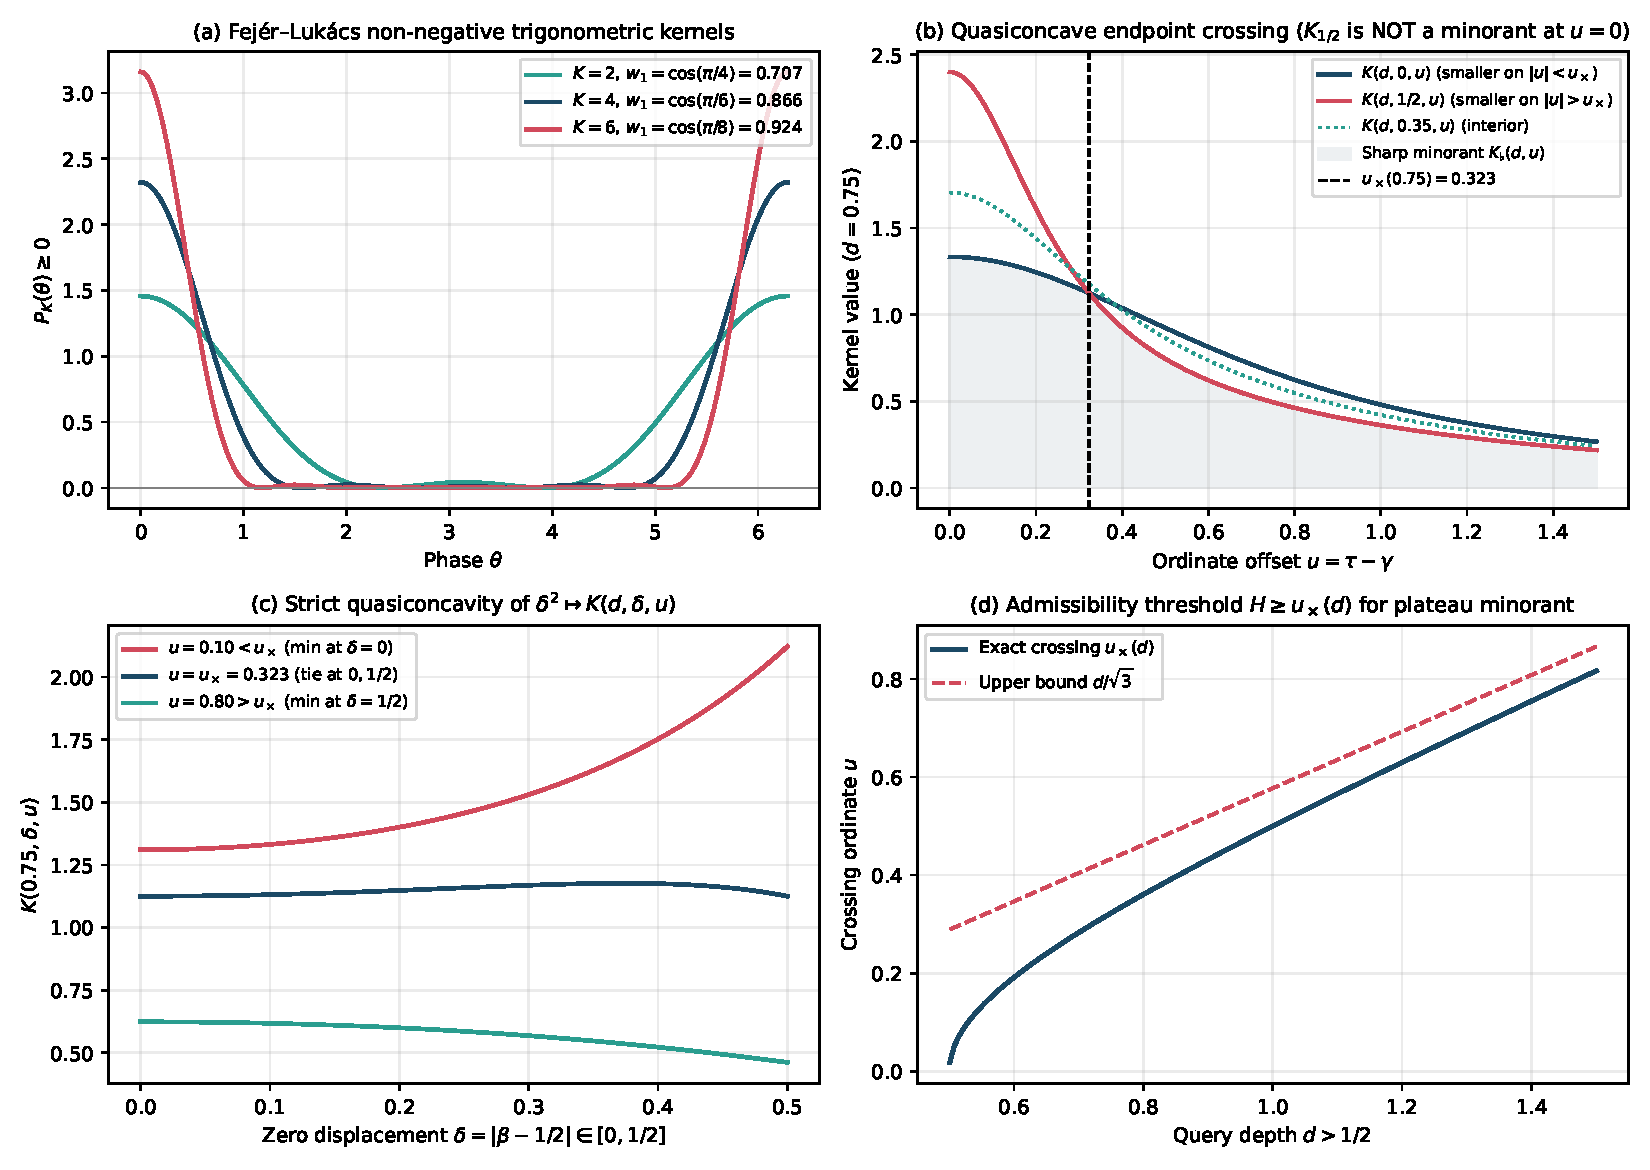
\includegraphics[width=0.95\textwidth]{figures/fig1_pure_square_and_sieved_strip_wall.pdf}
\caption{\textbf{(a)} Non-negative Fej\'er--Luk\'acs kernels $P_K(\theta) \ge 0$. \textbf{(b)} Crossing of $K(d,0,u)$ and $K(d,\frac{1}{2},u)$ at $u_{\times}(0.75) \approx 0.323$ ($K(d,\frac{1}{2},u)$ exceeds $K(d,0,u)$ on $\lvert u\rvert < u_{\times}$). \textbf{(c)} Quasiconcavity of $\delta^2 \mapsto K(0.75, \delta, u)$ across $[0, \frac{1}{2}]$. \textbf{(d)} Crossing threshold $u_{\times}(d) < d/\sqrt{3}$.}\label{fig:crossing_quasiconcave}
\end{figure}

\section{Rigorous Trudgian Stieltjes Bound and Smooth-Weight Comparison}\label{sec:trudgian}

Trudgian~\cite[Thm.~1]{trudgian2014} proved unconditionally for all $T \ge \ee$ that
\begin{equation}\label{eq:trudgian_2014_true}
\lvert S(T)\rvert \le B_S^{(0)}(T) := 0.112\ln T + 0.278\ln\ln T + 2.510.
\end{equation}
{\sloppy
In a constant-density toy model where $N'(\gamma)$ is frozen at $\frac{1}{2\pi}\ln(\tau/2\pi)$ on $\R$ and $\lvert S(\gamma)\rvert$ is frozen at $B_S^{(0)}(\tau)$, Stieltjes integration of $\widetilde{K}_H(d, \tau - \gamma)$ produces $\mathcal{F}_{\mathrm{model}}(d, \tau; H) := \frac{1}{2\pi}\ln\frac{\tau}{2\pi}[2HK_{\min}(d,H) + \pi - 2\Psi_{\mathrm{win}}(d,H)] - 2B_S^{(0)}(\tau)K_{\min}(d,H)$ ($K_{\min} := K(\cdot, \frac{1}{2}, \cdot)$, $\Psi_{\mathrm{win}}(d,H) := \int_0^H K_{\min}(d,u)\,\dd u$), whose $H$-derivative $[2H \cdot \frac{1}{2\pi}\ln(\tau/2\pi) - 2B_S^{(0)}(\tau)]\partial_H K_{\min}(d,H)$ vanishes at $H_{\mathrm{stat}}(\tau) := \frac{2\pi B_S^{(0)}(\tau)}{\ln(\tau/2\pi)}$ independently of $d$. Converting this heuristic into an unconditional inequality requires four rigorous corrections: (1)~the true Trudgian constant $2.510$ in~\eqref{eq:trudgian_2014_true}; (2)~logarithmic growth of $B_S^{(0)}(\gamma)$ on $[\tau+H, \infty)$; (3)~support $N(14) = 0$ and concavity of $\ln(\gamma/2\pi)$; and (4)~subtracting $2K_{\min}(d,H)$ at $k = 1$ so an extracted off-line pair $\{\rho_0, 1 - \bar{\rho}_0\}$ at $\gamma = t$ is not counted twice.\par}

\begin{theorem}[Unconditional Plateau Background Lower Bound]\label{thm:rigorous_stieltjes}
Let $d > \frac{1}{2}$, $\tau \ge 30$, $T_0 := 14$, $M := \frac{\tau}{2}$, and $u_{\times}(d) \le H \le M$. Set $\Phi_{\mathrm{plat}}(d,H;M) := 2HK_{\min}(d,H) + 2[\Psi_{\mathrm{win}}(d,M) - \Psi_{\mathrm{win}}(d,H)]$, $I_{2}(d,H;M) := \frac{1}{3}H^3 K_{\min}(d,H) + \int_H^M u^2 K_{\min}(d,u)\,\dd u$, and $c_{\mathrm{tail}}(x) := 0.112 + \frac{0.278}{\ln x}$. Then for any putative off-line pair $\mathcal{Z}_0 = \{\rho_0, 1 - \bar{\rho}_0\}$ at $\gamma = t$ (setting $\mathbf{1}_{\mathrm{focal}} = 1$ if $\tau = t$ and $0$ if $\mathcal{Z}_0 = \varnothing$ or $\tau \ne t$),
\begin{align}\label{eq:rigorous_bg_bound}
\sum_{\rho \notin \mathcal{Z}_0} K(d, d_\rho, \tau - \gamma) &\ge \mathcal{B}_{\mathrm{bg}}^{\mathrm{rig}}(d, \tau; H) \nonumber\\
&:= \left(\frac{1}{2\pi}\ln\frac{\tau}{2\pi} - \frac{1}{6\pi\tau^2}\right)\Phi_{\mathrm{plat}}(d,H;M) - \frac{2}{3\pi\tau^2}I_2(d,H;M) \\
&\quad - K_{\min}(d,\tau - T_0)\lvert S(T_0)\rvert - B_S^{(0)}(\tau - H)\bigl[K_{\min}(d,H) - K_{\min}(d,\tau - T_0)\bigr] \nonumber\\
&\quad - \bigl[B_S^{(0)}(\tau + H) + 2\mathbf{1}_{\mathrm{focal}}\bigr]K_{\min}(d,H) - \frac{c_{\mathrm{tail}}(\tau + H)}{\tau + H}\left(\frac{\pi}{2} - \Psi_{\mathrm{win}}(d,H)\right).\nonumber
\end{align}
\end{theorem}

\begin{proof}
Since $K(d, d_\rho, u) \ge \widetilde{K}_H(d, u) > 0$ for all $u \in \R$ by Theorem~\ref{thm:quasiconcave_crossing}(iii) and all zeros have $\lvert\gamma\rvert > 14$, dropping $\gamma < 0$ gives $\sum_{\rho \notin \mathcal{Z}_0} K(d, d_\rho, \tau - \gamma) \ge \int_{T_0}^{\infty} \widetilde{K}_H(d, \tau - \gamma)\,\dd N(\gamma) - 2\widetilde{K}_H(d,0)\mathbf{1}_{\mathrm{focal}}$. Using Backlund's identity $N(\gamma) = \frac{1}{\pi}\vartheta(\gamma) + 1 + S(\gamma)$ with $N(T_0) = 0$:
\begin{enumerate}[label=\textup{(\arabic*)},leftmargin=2.0em]
\item \textit{Smooth density integral.} Restricting $\int_{T_0}^{\infty} \widetilde{K}_H\frac{\vartheta'(\gamma)}{\pi}\,\dd\gamma$ to $[\tau - M, \tau + M] \subset [15, \infty)$ and pairing $\tau \pm u$ ($u \in [0, M]$) with Stirling's lower bound $\vartheta'(x) \ge \frac{1}{2}\ln\frac{x}{2\pi} - \frac{1}{24x^2} \ge \frac{1}{2}\ln\frac{x}{2\pi} - \frac{1}{6\tau^2}$ ($x \ge \frac{\tau}{2}$) and $\frac{1}{2}[\ln(\tau+u) + \ln(\tau-u)] = \ln\tau + \frac{1}{2}\ln(1 - \frac{u^2}{\tau^2}) \ge \ln\tau - \frac{2u^2}{3\tau^2}$ (since $\ln(1-w) \ge -\frac{4}{3}w$ on $[0, \frac{1}{4}]$) yields the first two terms of~\eqref{eq:rigorous_bg_bound}.
\item \textit{Stieltjes remainder.} Integrating $\int_{T_0}^{\infty} \widetilde{K}_H\,\dd S$ by parts ($\partial_\gamma\widetilde{K}_H \equiv 0$ on $(\tau-H, \tau+H)$, $> 0$ on $[T_0, \tau-H)$, and $< 0$ on $(\tau+H, \infty)$) bounds the left segment by $B_S^{(0)}(\tau-H)[K_{\min}(d,H) - K_{\min}(d,\tau-T_0)]$. On $[\tau+H, \infty)$, concavity of $\ln x$ and $\ln\ln x$ gives $B_S^{(0)}(\tau+u) \le B_S^{(0)}(\tau+H) + c_{\mathrm{tail}}(\tau+H)\ln(\frac{\tau+u}{\tau+H})$ for $u \ge H$; integrating $\ln(\frac{\tau+u}{\tau+H})(-\partial_u K_{\min}(d,u))$ by parts yields $\int_H^{\infty} \frac{K_{\min}(d,u)}{\tau+u}\,\dd u \le \frac{1}{\tau+H}(\frac{\pi}{2} - \Psi_{\mathrm{win}}(d,H))$.\qedhere
\end{enumerate}
\end{proof}

\begin{table}[t]
\centering
\caption{Zero-free region constant $R_{\mathrm{eff}}(t)$ ($\sigma \ge 1 - (R_{\mathrm{eff}}\ln t)^{-1}$) for the $K = 4$ Fej\'er--Luk\'acs polynomial without background subtraction vs.\ with the rigorous plateau bound~\eqref{eq:rigorous_bg_bound}, compared against Mossinghoff--Trudgian--Yang~\cite{mty2024} ($R = 5.558691$) and the equivalent Korobov--Vinogradov factor.}\label{tab:zfr_benchmarks}
\footnotesize
\setlength{\tabcolsep}{5.2pt}
\begin{tabular}{@{}ccccc@{}}
\toprule
Height $t$ & $R_{\mathrm{Stechkin}}(t)$ ($K=4$, no bg) & $R_{\mathrm{PlatRig}}(t)$ (Theorem~\ref{thm:rigorous_stieltjes}) & $R_{\mathrm{MTY}}$~\cite{mty2024} & $R_{\mathrm{KV,equiv}}(t)$~\cite{mty2024} \\
\midrule
$10^{6}$  & $14.7628$ & $12.8453$ & $5.558691$ & $31.7609$ \\
$10^{12}$ & $16.5113$ & $13.5060$ & $5.558691$ & $27.2560$ \\
$10^{20}$ & $17.2811$ & $13.4718$ & $5.558691$ & $24.1122$ \\
$10^{40}$ & $17.8964$ & $13.2316$ & $5.558691$ & $20.2291$ \\
\bottomrule
\end{tabular}
\end{table}

\begin{figure}[t]
\centering
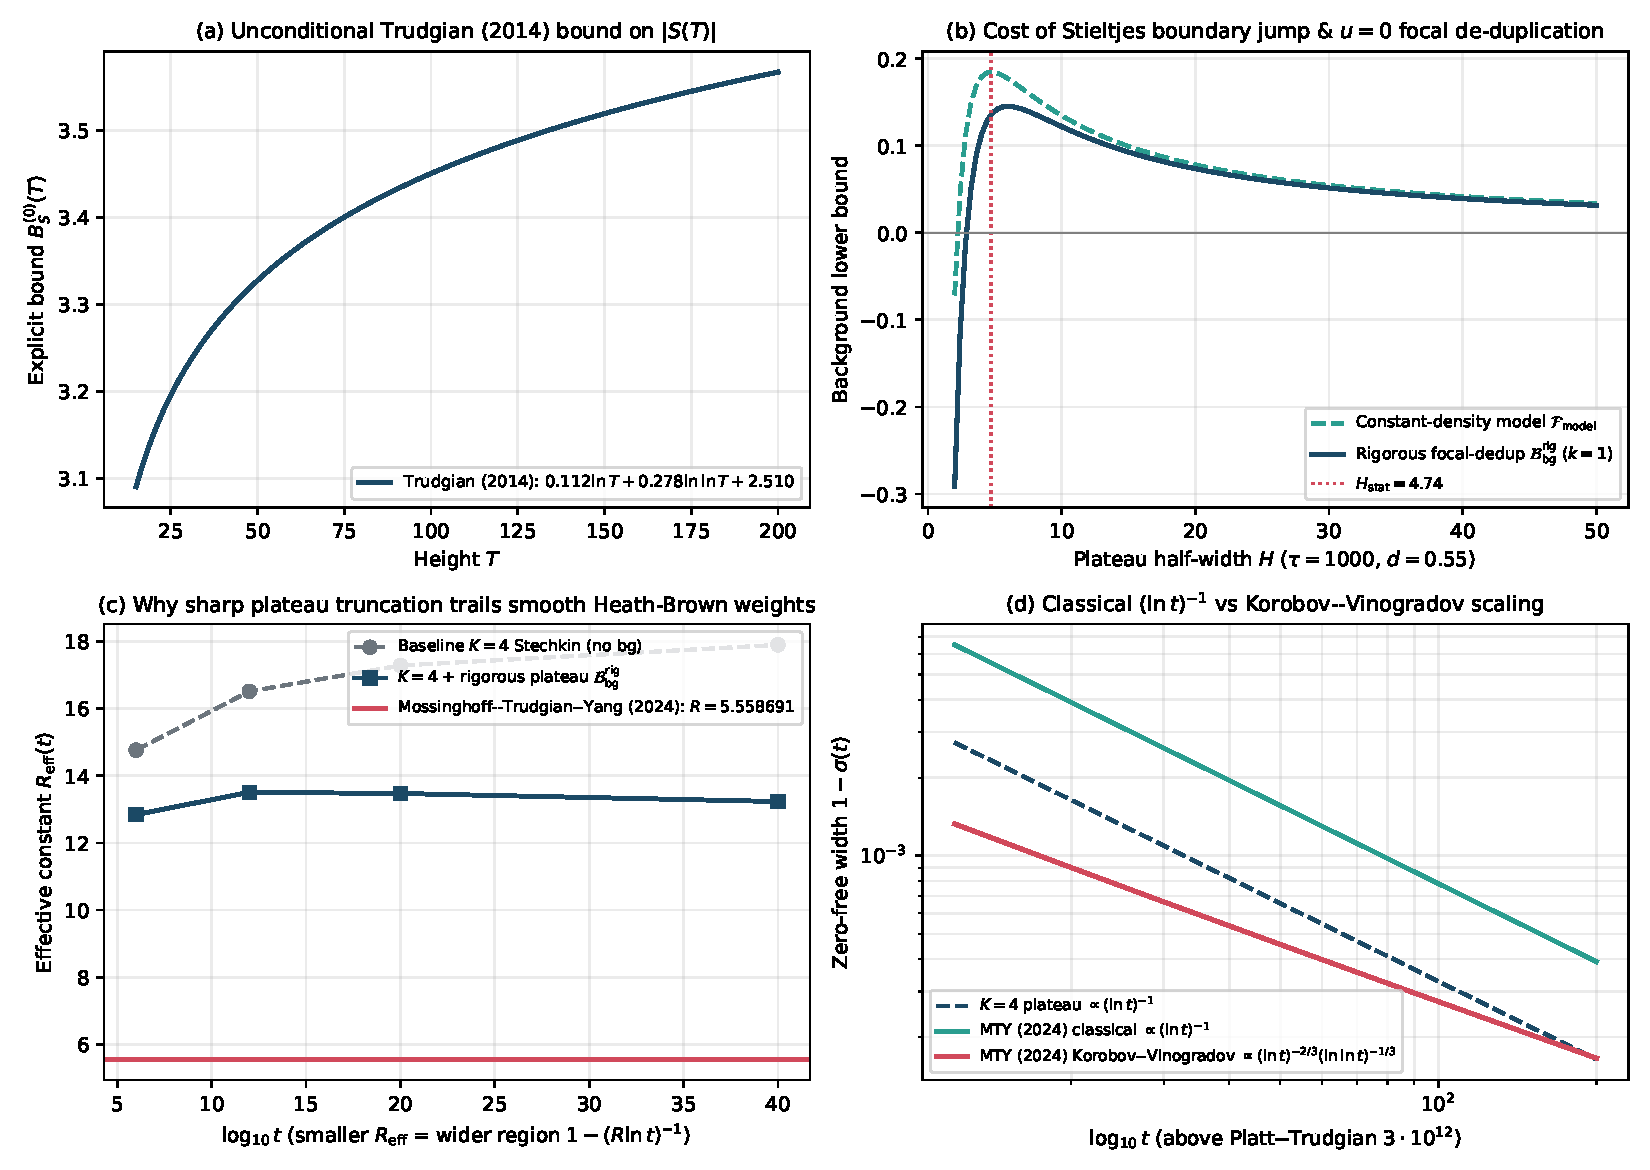
\includegraphics[width=0.95\textwidth]{figures/fig2_hadamard_conservation_and_stationary_variation.pdf}
\caption{\textbf{(a)} Unconditional Trudgian (2014) bound $B_S^{(0)}(T)$ with constant $2.510$. \textbf{(b)} Constant-density model $\mathcal{F}_{\mathrm{model}}$ vs.\ rigorous focal-deduplicated bound $\mathcal{B}_{\mathrm{bg}}^{\mathrm{rig}}$ at $\tau = 1000$. \textbf{(c)} Effective constant $R_{\mathrm{eff}}(t)$ compared with Mossinghoff--Trudgian--Yang ($R = 5.558691$). \textbf{(d)} Classical $(\ln t)^{-1}$ zero-free width vs.\ Korobov--Vinogradov scaling.}\label{fig:trudgian_benchmarks}
\end{figure}

\section{Scope, Boundary Conditions, and Open Questions}\label{sec:scope}

We summarize the methodological lessons established in Sections~\ref{sec:fejer}--\ref{sec:trudgian}:
\begin{enumerate}[label=\textup{(\arabic*)},leftmargin=2.2em]
\item \textit{Why sharp/plateau Poisson truncation trails smooth Heath-Brown weights.} As Table~\ref{tab:zfr_benchmarks} certifies, while $\mathcal{B}_{\mathrm{bg}}^{\mathrm{rig}}$ improves upon the baseline $K = 4$ Fej\'er--Toeplitz bound (reducing $R_{\mathrm{eff}}$ from $17.90$ to $13.23$ at $t = 10^{40}$), it remains substantially weaker than Mossinghoff--Trudgian--Yang's $R = 5.558691$~\cite{mty2024}. Two structural mechanisms explain this gap: first, $K_{\min}(d,u)$ has $\mathcal{O}(u^{-2})$ Lorentzian tails and slope discontinuities at $\lvert u\rvert = H$, incurring Stieltjes boundary penalties $\approx 2B_S^{(0)}(\tau)K_{\min}(d,H)$ plus focal de-duplication $-2K_{\min}(d,H)$; second, Heath-Brown's smooth compactly supported weight functions~\cite{heathbrown1992,mty2024} replace the raw Poisson kernel by rapidly decaying Mellin--Weil kernels whose derivatives are small everywhere, avoiding boundary jump penalties while jointly optimizing higher-degree cosine polynomials.
\item \textit{Asymptotic $(\ln t)^{-1}$ ceiling vs.\ Korobov--Vinogradov.} Every bounded-degree trigonometric inequality with $\sigma - 1 \asymp (\ln t)^{-1}$ yields at best a classical de la Vall\'ee Poussin width $\mathcal{O}((\ln t)^{-1})$; reaching $(\ln t)^{-2/3}(\ln\ln t)^{-1/3}$ requires Vinogradov--Korobov exponential-sum bounds on $\zeta(s)$~\cite{korobov1958,vinogradov1958,mty2024}. Moreover, for $\lvert t\rvert \le 3 \cdot 10^{12}$, all zeros already lie unconditionally on $\sigma = \frac{1}{2}$ by Platt--Trudgian~\cite{platttrudgian2021}.
\end{enumerate}

\appendix

\section{Numerical and Interval Certification Protocols}\label{app:interval}

{\sloppy
In the standalone suite \texttt{scripts/\allowbreak verify\_\allowbreak paper7\_\allowbreak mirror\_\allowbreak hadamard\_\allowbreak variation.py}, all identities and bounds are verified in 50-decimal arithmetic (\texttt{mpmath.mp.dps = 50}) and 35-digit interval arithmetic (\texttt{mpmath.iv.dps = 35}):\par}
\begin{enumerate}[label=\textup{(\arabic*)},leftmargin=2.2em]
\item \textit{Quasiconcave crossing certification.} Across $d \in \{0.55, 0.75, 1.00, 1.50\}$, $\lvert K(d,0,u_{\times}) - K(d,\frac{1}{2},u_{\times})\rvert < 10^{-47}$, $K(d,0,0) - K(d,\frac{1}{2},0) < 0$, and interval arithmetic encloses $u_{\times}(0.60) \in [0.19148542, 0.19148543] < 0.60/\sqrt{3}$.
\item \textit{Validation against exact Riemann zeros.} Summing $K(d, 0, \tau \mp \gamma_n)$ over the first $220$ critical-line ordinates strictly exceeds $\mathcal{B}_{\mathrm{bg}}^{\mathrm{rig}}(d, \tau; H)$ at all test points $(d, \tau, H)$.
\end{enumerate}

\section*{Use of AI and computational verification}

{\sloppy
In accordance with editorial policies on transparency in scientific computing, the author discloses that the AI research assistant \textbf{Gemini} (Google DeepMind) assisted in uncovering the $\lvert u\rvert < u_{\times}(d)$ crossing of $K(d,\frac{1}{2},u)$, proving quasiconcavity of $\delta^2 \mapsto K(d,\delta,u)$, correcting the Stieltjes tail, concavity, and focal de-duplication terms, and implementing \texttt{scripts/}\allowbreak\texttt{\detokenize{verify_paper7_mirror_hadamard_variation.py}} (exit code~$0$).\par}

\begin{thebibliography}{99}

\bibitem{csordas1986}
G.~Csordas, T.~S.~Norfolk, and R.~S.~Varga,
\emph{The Riemann hypothesis and the Tur\'an inequalities},
Trans. Amer. Math. Soc. \textbf{296} (1986), no.~2, 521--541.

\bibitem{dlvp1899}
C.-J.~de~la~Vall\'ee~Poussin,
\emph{Sur la fonction $\zeta(s)$ de Riemann et le nombre des nombres premiers inf\'erieurs \`a une limite donn\'ee},
M\'em. Couronn\'es Autres M\'em. Publ. Acad. Roy. Sci. Lett. Beaux-Arts Belg. \textbf{59} (1899), 1--74.

\bibitem{fejer1916}
L.~Fej\'er,
\emph{\"Uber trigonometrische Polynome},
J. Reine Angew. Math. \textbf{146} (1916), 53--82.

\bibitem{heathbrown1992}
D.~R.~Heath-Brown,
\emph{Zero-free regions for Dirichlet $L$-functions, and the least prime in an arithmetic progression},
Proc. London Math. Soc. (3) \textbf{64} (1992), 265--338.

\bibitem{hinkkanen1997}
A.~Hinkkanen,
\emph{On functions of bounded type},
Complex Variables Theory Appl. \textbf{34} (1997), 119--139.

\bibitem{hudson1974}
R.~L.~Hudson,
\emph{When is the Wigner quasi-probability density non-negative?},
Rep. Math. Phys. \textbf{6} (1974), no.~2, 249--252.

\bibitem{jacobi1829}
C.~G.~J.~Jacobi,
\emph{Fundamenta Nova Theoriae Functionum Ellipticarum},
Borntraeger, K\"onigsberg, 1829.

\bibitem{kondratiev1977}
V.~P.~Kondrat'ev,
\emph{On some extremal properties of positive trigonometric polynomials},
Mat. Zametki \textbf{22} (1977), no.~3, 371--374.

\bibitem{korobov1958}
N.~M.~Korobov,
\emph{Estimates of trigonometric sums and their applications},
Uspekhi Mat. Nauk \textbf{13} (1958), no.~4, 185--192.

\bibitem{lagarias1999}
J.~C.~Lagarias,
\emph{On a positivity property of the Riemann $\xi$-function},
Acta Arith. \textbf{89} (1999), no.~3, 217--234.

\bibitem{missiaen2026p5}
T.~Missiaen,
\emph{Logarithmic dilation of the Jacobi--Riemann kernel, strip-holomorphic shell partitions, Stieltjes diagonal asymptotics, and off-diagonal obstructions},
Preprint, Paper~V in this series, 2026.

\bibitem{missiaen2026p6}
T.~Missiaen,
\emph{Sieved mirror kernels, Gonek--Hughes--Keating versus entire exponential prime factors, prime-power purity on $(X, X^2]$, and functional-equation obstructions},
Preprint, Paper~VI in this series, 2026.

\bibitem{mty2024}
M.~J.~Mossinghoff, T.~S.~Trudgian, and A.~Yang,
\emph{Explicit zero-free regions for the Riemann zeta-function},
Res. Number Theory \textbf{10} (2024), Art.~11.

\bibitem{platttrudgian2021}
D.~J.~Platt and T.~S.~Trudgian,
\emph{The Riemann hypothesis is true up to $3\cdot 10^{12}$},
Bull. Lond. Math. Soc. \textbf{53} (2021), no.~3, 792--797.

\bibitem{polya1926}
G.~P\'olya,
\emph{Bemerkung \"uber die Integraldarstellung der Riemannschen $\xi$-Funktion},
Acta Math. \textbf{48} (1926), 305--317.

\bibitem{riemann1859}
B.~Riemann,
\emph{Ueber die Anzahl der Primzahlen unter einer gegebenen Gr\"osse},
Monatsber. K\"onigl. Preuss. Akad. Wiss. Berlin (1859), 671--680.

\bibitem{speiser1934}
A.~Speiser,
\emph{Geometrisches zur Riemannschen Zetafunktion},
Math. Ann. \textbf{110} (1934), 514--521.

\bibitem{stechkin1970}
S.~B.~Stechkin,
\emph{Zeros of the Riemann zeta-function},
Mat. Zametki \textbf{8} (1970), 419--429; English transl. in Math. Notes \textbf{8} (1970), 706--711.

\bibitem{szego1975}
G.~Szeg\H{o},
\emph{Orthogonal Polynomials},
4th ed., Amer. Math. Soc., Providence, RI, 1975.

\bibitem{trudgian2014}
T.~S.~Trudgian,
\emph{An improved upper bound for the argument of the Riemann zeta-function on the critical line II},
J. Number Theory \textbf{134} (2014), 280--292.

\bibitem{vinogradov1958}
I.~M.~Vinogradov,
\emph{A new estimate of the function $\zeta(1 + \ii t)$},
Izv. Akad. Nauk SSSR Ser. Mat. \textbf{22} (1958), 161--164.

\bibitem{wigner1932}
E.~P.~Wigner,
\emph{On the quantum correction for thermodynamic equilibrium},
Phys. Rev. \textbf{40} (1932), 749--759.

\end{thebibliography}

\end{document}
